\documentclass[assignment03_Solutions]{subfiles}

\IfSubStr{\jobname}{\detokenize{Solutions}}{\toggletrue{solutions}}{\toggletrue{solutions}}

\fancypagestyle{firstpage}

{\rhead{Assignment 3 \linebreak \textit{Version: \today}}}

\title{Assignment 3: Probability and Fairness, Text Classification}
\author{Machine Learning}
\date{Fall 2019}
\invalidatemargin

\begin{document}

\maketitle
\thispagestyle{firstpage}


\begin{learningobjectives}
\bi
\item TODO
\ei
\end{learningobjectives}

\section{Bayesian Networks and Algorithmic Fairness}

TODO: (make sure to describe limitations upfront).  Maybe link to resource.  This should be 30 minutes long.

\section{Maximum Likelihood Parameter Estimation for Discrete Models}
Last assignment, we met the Na\"ive Bayes model.  As a motivating example, we presented a BN for the Titanic Dataset that conceptualized three features (\emph{male}, \emph{is young}, and \emph{fare class}) being generated by whether or not the passenger survived.  Here is the BN corresponding to this model.

\begin{center}
\includegraphics[width=0.8\linewidth]{../02/figures/titanicbn}
\end{center}

In the last assignment, we gave a high-level description of how we determined the parameters in the conditional probability tables.
\begin{quote}
The probabilities in this BN were computed by looking at the training set and counting the appropriate passengers that fell into each category.  For instance, to compute $p(\mathcal{Y}|\mathcal{S})$ since $p(\mathcal{Y}|\mathcal{S}) = \frac{p(\mathcal{Y}, \mathcal{S})}{p(\mathcal{S})}$, we can approximate this probability by counting the number of passengers under 5 who survived and dividing by the total number who survived (note that there are some subtle and important modifications to this method of fitting these probabilities that we'll discuss in the next assignment).  This process was repeated for each conditional probability.  Since we assume that all of the features are conditionally independent given the output ($\mathcal{S}$ in this case), this process is done independently for each feature.
\end{quote}

While this seems totally logically, it helps to be rigorous about \emph{why} these were the right probabilities given the training data.  In this section, we'll go over the math behind determining these probabilities.  The goal will be to provide a general outline of a process for fitting parameters of a BN to data through exercising that process on a pretty basic model (the Titanic BN shown above).

\subsection{Formalizing the Problem}
We can think of the probabilities in the conditional probability tables as the parameters of our Na\"ive Bayes model.  The basic idea is that we're going to use some training data in order to fit the parameters of our model to agree as closely as possible with the training data.  This should feel pretty familiar to you.  In the last module we did this again and again by tuning the model parameters to fit the training outputs given the training inputs (in the last module the parameters were typically weights of a neural network or logistic regression model).  We'll be doing something very similar here, so hopefully what you learned in the last module will help to learn this new idea.

Suppose we are given $n$ training data points $\mathbf{x_1}, \mathbf{x_2}, \ldots, \mathbf{x_n}$.  In the case of the titanic dataset $\mathbf{x_i}$ would be a four-dimensional vector consisting of the following information: whether the passenger survived ($\mathcal{S}$), the passenger's fare class ($\mathcal{C}$), whether the passenger was male ($\mathcal{M}$), and whether the passenger was under the age of 5 ($\mathcal{Y}$).  Further, suppose we have a model is parameterized byline some parameters $\mathbf{\Theta}$ that computes the probability of any input $\mathbf{x}$.  For instance, our model can compute $p(\mathbf{x_i} | \mathbf{\Theta})$.  For any of our training points (or any other possible input for that matter).

\begin{understandingcheck}
In the case of the Titanic model, what would the parameters $\mathbf{\Theta}$ represent? (check solutions for the answer if you get stuck).
\begin{boxedsolution}
The parameters in this case would represent all of the entries in the conditional probability tables in the BN.  For example, the parameters would encode $p(\mathcal{S}$, $p(\mathcal{M}|\mathcal{S})$, etc.
\end{boxedsolution}
\end{understandingcheck}

Given the our model of $p(\mathbf{x_i}|\mathbf{\Theta})$, we would now like to fit (or estimate) the parameters, $\mathbf{\Theta}$, to the training data.  To do this, we can use the technique of maximum likelihood estimation.  The maximum likelihood estimate of the parameters is given by the following formula.

\begin{align}
\mathbf{\Theta^\star} &= \argmax_{\mathbf{\Theta}} p(\mathbf{x_1}, \mathbf{x_2}, \ldots \mathbf{x_n} | \mathbf{\Theta}) \label{eq:mle}
\end{align}

Intuitively, Equation~\ref{eq:mle} captures the idea that we should choose the model parameters that makes the observed training data as likely as possible under our model.

\subsection{Simplifications to Equation~\ref{eq:mle}}

It may seem that computing the probability in Equation~\ref{eq:mle} would be quite difficult.   While in some cases it can be, there are some reasonable simplifying assumptions that we can apply to make it a little bit easier,  Later we will show how this can be applied to the Na\"ive Bayes algorithm.  One of the most common assumptions in machine learning is to assume that our training data points are conditionally independent given $\mathbf{\Theta}$ (that is $\mathbf{x_i} \condindep \mathbf{x_j}~|~\mathbf{\Theta}$ for all $i \neq j$).

\begin{understandingcheck}
Todo
\end{understandingcheck}

If we apply this conditional independence assumption to Equation~\ref{eq:mle}, we derive the following equation.

\begin{align}
\mathbf{\Theta^\star} &= \argmax_{\mathbf{\Theta}} p(\mathbf{x_1} |  \mathbf{\Theta}) p(\mathbf{x_2} | \mathbf{\Theta}) \ldots p(\mathbf{x_n} | \mathbf{\Theta}) \label{eq:mleiid}
\end{align}

To make our leaves even easier, we can apply a log to the thing we are maximizing without changing the $\argmax$ (this works because $\log$ is a monotonic (continuously increasing function.  That is, $\argmax_x f(x) = \argmax_x \log \left ( f(x) \right)$).


\begin{align}
\mathbf{\Theta^\star} &= \argmax_{\mathbf{\Theta}} \log \left ( p(\mathbf{x_1} |  \mathbf{\Theta}) p(\mathbf{x_2} | \mathbf{\Theta}) \ldots p(\mathbf{x_n} | \mathbf{\Theta})  \right) \nonumber \\
&=  \argmax_{\mathbf{\Theta}} \sum_{i=1}^n \log p(\mathbf{x_i} |  \mathbf{\Theta})  \label{eq:mleiidlog}
\end{align}

The importance of applying the log might not be apparent yet, but it actually did some very useful work for us.  It allowed us to break apart our probability into multiple components (one for each data point).  We can now optimize the sum of a bunch of functions rather than the product (which turns out to be much easier).  We'll see how this plays out in the next section.

\subsection{Maximum Likelihood Estimation for Na\"ive Bayes}

In this section we'll be applying the technique of maximum likelihood estimation (MLE) to the Na\"ive Bayes algorithm.  We'll also connect it back to the Titanic model to see how our general technique matches with our intuition regarding how to fit parameters to passenger survival data.

\vspace{1em}
\begin{exercise}[(60 minutes)]
The BN for the Na\"ive Bayes model is shown below.

\begin{center}
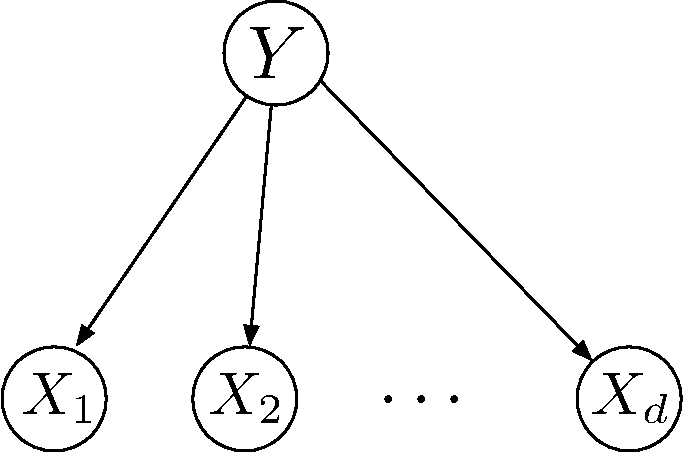
\includegraphics[width=0.3\linewidth]{figures/naivebayesgm}
\end{center}

In this BN, the variable $\mathcal{Y}$ represents some category of interest (e.g., survive versus not survive), and $X_1, X_2, \ldots, X_d$ represent various features of a particular data instance (e.g., age, sex, fare class).  The rules of d-separation tell us that $X_i \condindep X_j~|~Y$ for all $i \neq j$.  For simplicity, we'll assume that $Y$ takes on values from the set $\{1, 2, \ldots c \}$ and each of the $X_i$ takes on values form the set $\{1, 2, \ldots, r\}$.  Extending this to the case where each of the random variables takes values from some other discrete set is straightforward.

%Suppose we want to apply the technique of maximum likelihood estimation to the Na\"ive Bayes model.  For training data you are given a training set of input output pairs as $\left (\mathbf{x_1}, y_1 \right),  \left (\mathbf{x_2}, y_2 \right), \ldots, \left (\mathbf{x_n}, y_n \right)$.  Each $\mathbf{x_i}$ represents a $d$ dimensional vector that corresponds to the values of the random variables, $X$, in the BN (e.g., the $j$ the random variable in the BN $X_j$ for the $i$th data point would equal $x_{i,j}$).  Each $y_i$ represents a value for the random variable $Y$ in the bn (e.g., the random variable $Y$ for the $i$th data point would equal $y_i$).

\bes
\item Equation~\ref{eq:mleiidlog} can be written for this model as
\begin{align}
\mathbf{\Theta^\star} &= \argmax_{\Theta} \sum_{i=1}^n \log p(X_1 = x_{i,1}, X_2 = x_{i,2}, \ldots, X_d = x_{i,d}, Y = y_i | \mathbf{\Theta}) \enspace . \label{eq:nbmle}
\end{align}
Using the concept of d-separation on the BN graph for Na\"ive Bayes (the figure above), simplify Equation~\ref{eq:nbmle}.  Hint: you'll want to break apart the big joint probability (the probability of all fo the $X_i$'s and $Y$ using conditional independence).

Warning: spoiler alert if you look at part b.
\begin{boxedsolution}
We know that each of the variables in a BN is conditionally independent given its parents.  We can use this result to write the joint probability of all of our random variables the $X$'s and $Y$ in terms of the probability of each conditioned on its parents.
\begin{align}
\mathbf{\Theta^\star} &= \argmax_{\mathbf{\Theta}} \sum_{i=1}^n  \left ( \log p(Y = y_i)  + \sum_{j=1}^d \log p(X_j = x_{i,j} | Y = y_i,  \mathbf{\Theta}) \right ) \enspace . \label{eq:nbmle}
\end{align}
\end{boxedsolution}

\item The answer to part (a) is given here to help setup the next part of this question.

\begin{align}
\mathbf{\Theta^\star} &= \argmax_{\mathbf{\Theta}} \sum_{i=1}^n  \left ( \log p(Y = y_i)  + \sum_{j=1}^d \log p(X_j = x_{i,j} | Y = y_i,  \mathbf{\Theta}) \right ) \enspace . \label{eq:nbmle}
\end{align}

Suppose, $\Theta$ consists of the following parameters. (TODO: replace everything with $\theta$ instead of $q$).

\bi
\item $q(1), q(2), \ldots, q(c)$ represent the prior probability that $y$ takes on a particular value (e.g., $q_i = p(Y = i)$).  Note that in order for $q_1, \ldots, q_c$ to represent a valid probability mass function (PMF) $\sum_{i=1}^c p_i = 1$.
\item $q_{j}(k | i)$ represents the conditional probability that feature $X_j$ takes on value $k$ given $Y = i$.  That is $q_{j}(k | j) = p(X_j = k | Y = i)$.  In order for the $q_j(k|i)$'s to represent valid PMFs, $\sum_{k=1}^{r} q_{j}(k | j) = 1$.
\ei

Suppose that $\mbox{ycount}(i)$ represents the number of training points that have $y = i$ (that is $\mbox{ycount}(i) = \sum_{j=1}^n \mathbb{I} \left [y_j = i \right]$ where $\mathbb{I}$ is the indicator function that returns 1 if the condition is true and 0 otherwise).

Suppose that $\mbox{xcount}_j(k|i)$ represents the number of training points that had $x_j = k$ and $y = i$ (that is $\mbox{xcount}_j (k|i) = \sum_{k=1}^n \mathbb{I} \left [ x_j = k, y_j = i \right ]$).

Rewrite Equation~\ref{eq:nbmle} in terms of the $q(i)$'s, $q_{j}(k|i)$'s, $\mbox{ycount}$'s, and $\mbox{xcount}$'s.  Hint: replace summations over the data points with summations over the possible values that the random variables can take on.

Warning: spoiler alert if you look at part c.
\begin{boxedsolution}
\begin{align}
\mathbf{\Theta}^\star &= \argmax_{\mathbf{\Theta}} \left ( \sum_{i=1}^c \mbox{ycount}(i) \log q(i)  \right) +  \left ( \sum_{j=1}^d \sum_{i=1}^c \sum_{k=1}^r \mbox{xcount}_j(k|i) \log q_j(k|i) \right )
\end{align}
\end{boxedsolution}

\item The maximum likelihood equation for the model (part b) is as follows.
\begin{align}
\mathbf{\Theta}^\star &= \argmax_{\mathbf{\Theta}} \left ( \sum_{i=1}^c \mbox{ycount}(i) \log q(i)  \right) +  \left ( \sum_{j=1}^d \sum_{i=1}^c \sum_{k=1}^r \mbox{xcount}_j(k|i) \log q_j(k|i) \right ) \label{eq:mleparameterized}
\end{align}

Since each of the terms in these summations only depends on a subset of the parameters, we can break the equation apart into a bunch of separate maximum likelihood estimation problems.

\begin{align}
q^\star(1), \ldots, q^\star(c)&= \argmax_{q(1), \ldots, q(c)}\sum_{i=1}^c \mbox{ycount}(i) \log q(i) \label{eq:qmarginals}
\end{align}

This equation is subject to the constraint that $\sum_{i=1}^c q(i) = 1$ and each $q(i) \geq 0$ (since these must form a valid PMF).

Additionally, for $i$ from 1 to $c$ and $j$ from 1 to $d$
\begin{align}
q_j^\star(1|i), \ldots, q^\star_j(r|i) &= \argmax_{q_j(1|i), \ldots, q_j(r|i)}\sum_{k=1}^r \mbox{xcount}_j(k|i) \log q_j(k|i) \enspace . \label{eq:qconditionals}
\end{align}
These equation are subject to the constraint that $\sum_{k=1}^r q_j(k|i) = 1$  and each $q_j(k|i) \geq 0$ (since these must form a valid PMF).


Each of these optimization problems is what is known as a constrained optimization problem.  It is an optimization problem since we are looking to maximize a function and it is a constrained optimization problem since we must ensure that the solution satisfies the constraint that the relevant $q$'s are all non-negative and add up to 1.

If you'd like to derive the solution to these constrained optimization problems, you would use the technique of \href{http://tutorial.math.lamar.edu/Classes/CalcIII/LagrangeMultipliers.aspx}{Lagrange Multipliers}.  Also, here is \href{http://www.cs.columbia.edu/~mcollins/em.pdf}{a walkthrough of using this strategy to solve the equations for the Na\"ive Bayes algorithm} (the proof is in section 4.2).  Instead of having you prove this directly, let's take as given the following theorem.

Suppose $c_1, \ldots c_m$ represent non-negative constants ($c_i \neq 0)$.  Further, suppose $q_1, \ldots q_m$ represents a PMF ($q_i \geq 0$ and $\sum_{i=1}^m q_i = 1$).  If this is true then,

\begin{align}
q^\star_1, \ldots, q^\star_m &= \argmax_{q_1, \ldots, q_m} \sum_{i=1}^m c_i \log q_i \nonumber \\
q^\star_i &= \frac{c_i}{\sum_{i=1}^m c_i} \label{eq:multinomial}
\end{align}

Using the result above, find the optimal values of the parameters of the Na\"ive Bayes model (i.e., compute $q^\star(1), \ldots, q^\star(c)$ and $q_j^\star(1|i), \ldots, q^\star_j(r|i))$).  Does the result match your intuitions about what the $q$ values should be?

Hint: You should be able to pattern match Equation~\ref{eq:multinomial} to both Equation~\ref{eq:qmarginals} and Equation~\ref{eq:qconditionals}. 

\begin{boxedsolution}
Equation~\ref{eq:qmarginals} can be solved using Equation~\ref{eq:multinomial} in the following way.
\begin{align}
q^\star(i) &= \frac{\mbox{ycount}(i)}{\sum_{j=1}^c \mbox{ycount}(j)}
\end{align}

Equation~\ref{eq:qconditionals} can be solved using Equation~\ref{eq:multinomial} in the following way.
\begin{align}
q_j^\star(k|i) &= \frac{\mbox{xcount}_j(k|i)}{\sum_{u=1}^r \mbox{xcount}_j(u|i)}
\end{align}
\end{boxedsolution}


\ees


\end{exercise}

\section{Text Classification with Bag of Words}
Next we'll be applying Na\"ive Bayes to the task of classifying text.

\begin{externalresources}[(45 minutes)]
This will be done in the Assignment 3 companion notebook.
\end{externalresources}

\section{The Intelligent Design of Jenny Chow}

This assignment is fully described on the \href{https://canvas.instructure.com/courses/1659968/assignments/12785465?module_item_id=26196347}{Intelligent Design of Jenny Chow Canvas page}.  There is also an alternative described on the assignment page if you can't attend.  Make sure to look at the assignment before going to the play since we are asking you to capture some of your reactions / thoughts so that you can bring them to class on Monday for discussion.

\end{document}
